\begin{figure}[htbp]
\centering
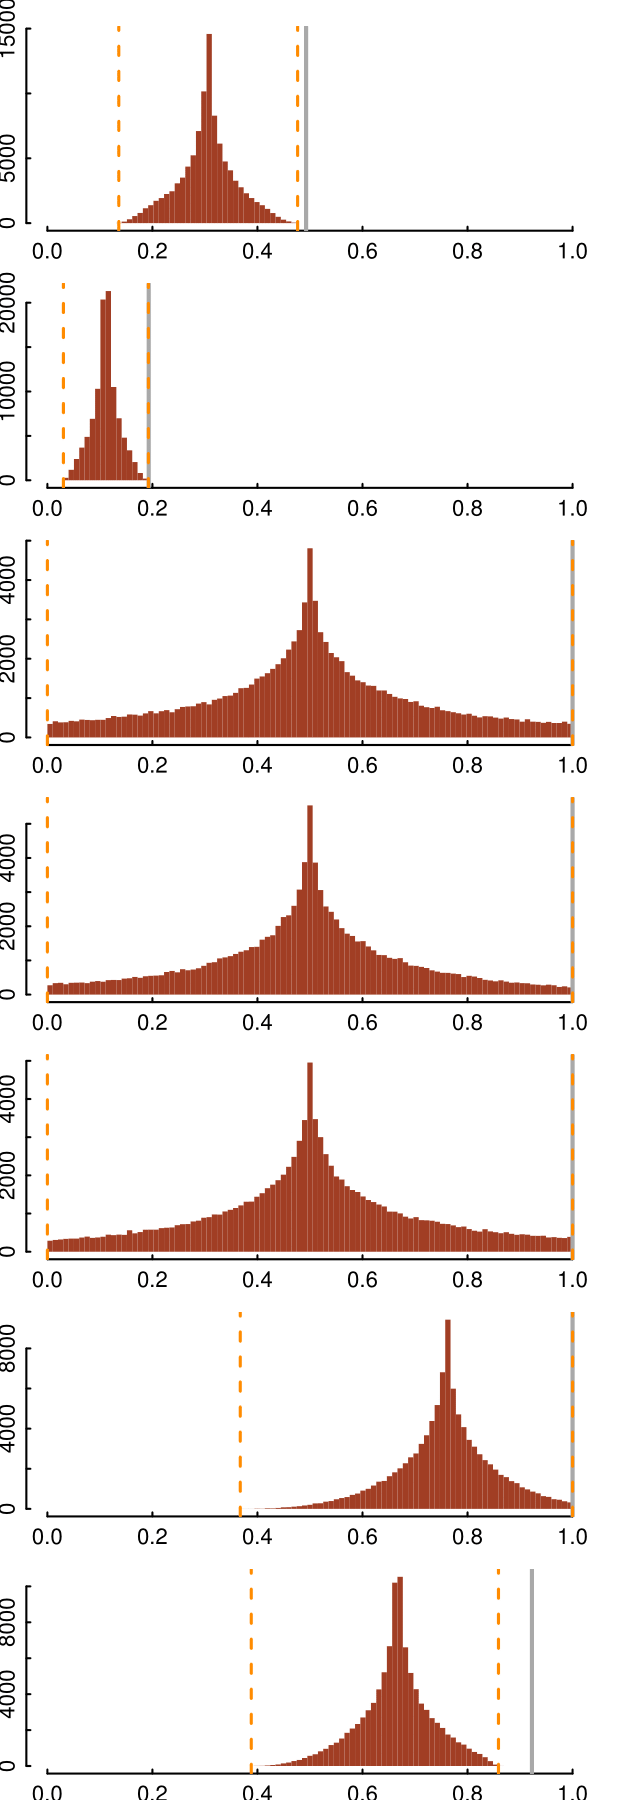
\includegraphics[width=7.5cmh]{sections/figs/raw_histograms.png}
\caption{After sampling of the feasible activation set, we show histograms of each muscle's activaiton across all solutions. For this set of distributions, the task was 50\% of maximal force output in the palmar direction.}
\label{fig:raw_histograms}
\end{figure}


\section{RESULTS}

Figure \ref{fig:raw_histograms} shows the distributions of activations resulting from $1,000,000$ solutions computed with Hit-and-Run sampling. This is the first time (to our knowledge) that the internal structure of the feasible activation set has been visualized for a sub-maximal force.

Notice also that the lower and upper bounds of the activations (i.e., the dashed lines that indicate their bounding box), are unhelpful in determining the actual density distribution of feasible activations.
Note also that the activation needed for the maximal force output (thick gray line) is very often not the mode of the activations at 50\% of output.

